% \begingroup
% \let\clearpage\relax
% \chapter{解决方案}
% \section{问题描述}
% 给定训练集 $D^{train} = \{(x_t,y_t)\}^{T}_{t=1}$ ,基学习器 $A$ 的目标是利用参数 $\theta$ 对预测器 $y=f(x,\theta)$ 进行估计,
% 以在未见的测试集 $D^{test} = \{(x_a, y_a)\}^{Q}_{t=1}$ 上实现更好的泛化能力,
% % 通常假设训练集和测试集采样自相同分布,并使用参数 $\phi$的嵌入模型$f_{\phi}$将样本域映射到特征空间。
% % 对于基于优化的学习器,参数通过最小化训练数据上的经验损失以及正则项获得。
% \begin{equation}
%     \label{equation:1}
%     \theta = A(D^{train}; \phi) = \mathrm{arg\,min}_{\theta}L^{base}(D^{train}; \theta, \phi) + R(\theta)
% \end{equation}
% 其中,$L^{base}$ 是损失函数,$R(\theta)$ 是正则项,在训练数据有限的情况下,正则项在模型的泛化方面扮演很重要的角色。

% 为了最小化泛化误差,少样本元学习方法旨在学习任务分布中的最优模型,这可以看作是在一个任务集合上进行学习:
% $T = \{(D_{i}^{train}, D_{i}^{test})\}^{I}_{i=1}$,通常被称为元训练集。
% % 通过元组$(D_i^{train}, D_i^{test})$描述的训练和测试数据集。
% 本文的目标是学习一个嵌入模型$\phi$,使得在给定基础学习者$A$的情况下,在不同任务中达到最小化泛化(或测试)误差的效果。

% 为了实现这一目标,本文的学习目标是:
% \begin{equation}
%     \label{equation:2}
%     \min_{\phi} \mathbb{E}_{T} [L^{meta}(D^{test}; \theta, \phi), \mathrm{where} \, \theta = A(D^{train}, \phi)]
% \end{equation}

% \begin{figure}[htbp]
%     \centering
%     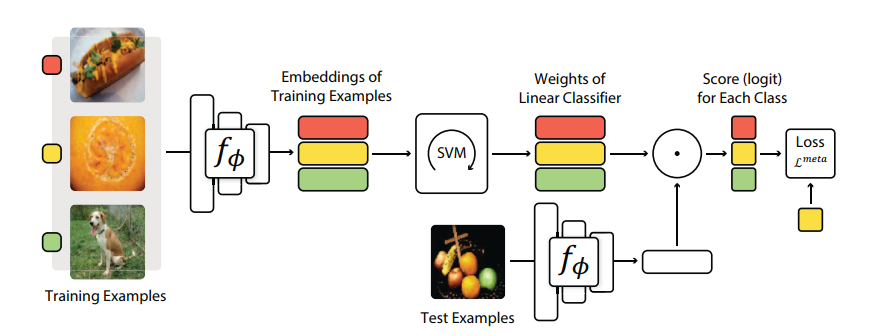
\includegraphics[width=.7\linewidth]{figure/p1.png}
%     \caption{Overview of our approach.}
%     \label{fig:1}
% \end{figure}

% 图\ref{fig:1} 展示了单一任务的训练和测试过程。一旦学习到嵌入模型 $f_{\phi}$,它的泛化性能可以在一个保留的任务集合(通常称为元测试集)上进行评估。元测试集 
% $S = \{(D_j^{train}, D_j^{test})\}^J_{j=1}$ 可以用公式来计算:
% \begin{equation}
%     \label{equation:3}
%     \mathbb{E}_S[L^{meta}(D^{test}; \theta, \phi), \mathrm{where} \, \theta = A(D^{train}; \phi)]
% \end{equation}

% 根据之前的研究\upcite{ravi2017optimization,finn2017model},公式 \ref{equation:2} 和 公式\ref{equation:3}
% 中期望值的估计分别被称为元训练和元测试阶段。
% 在元训练阶段,本文会保留一个额外的验证集来选择元学习器的超参数并挑选最佳的嵌入模型。

% % \section{创新思想}
% % 本文将可微的二次规划求解器和不同的线性分类器综合起来。利用以上两个特性,本文实现了在
% % 计算成本略有增加的情况下提供了比最临近分类器更大的收益。

% % 本文利用线性分类器的凸优化性质,将线性分类器作为基础学习器应用于元学习,用于解决可计算性问题。


% \section{具体方法}
% \subsection{任务集}
% 少样本学习使用K-way,N-shot分类任务对模型进行评估,
% 其中K表示类别数,$N$表示每个类别的训练样本数,通常取较小的值,
% % 如$N\in{1,5}$。
% % 虽然 miniImageNet\upcite{ravi2017optimization} 等数据集没有明确给出训练集和测试集$(D_i^{train}, D_i^{test})$,
% 每个元学习任务可以在元训练阶段即兴构建,这被称为任务集。
% 一个任务集 $\tau_i=(D_i^{train}, D_i^{test})$ 可以按以下方式进行采样\upcite{ravi2017optimization,vinyals2016matching}:

% 总体类集为$C^{train}$, 对于每个任务集,首先类$C_i$(包含来自$C^{train}$的K类)被有放回抽样得到,
% 训练集$D_i^{train} = \{(x_n, y_n) | n=1,...,N \times K, y_n \in C_i\}$(每个类包含N个图像)被采样,
% 测试集$D_i^{test} = \{(x_n, y_n) | n = 1,...,Q \times K, y_n \in C_i\}$(每个类包含Q个图像)被采样。

% 需要无放回抽样,如$D_i^{train} \cap D_i^{test} = \emptyset $,以优化泛化误差。以同样的方式从$C^{val}$
% 和$C^{test}$各自即兴构造元验证集(meta-validation)和元测试集(meta-test)。
% 为了度量嵌入模型对未见类的泛化,$C^{train}, C^{val}, C^{test}$需被互斥选择。

% \subsection{凸基学习器}

% % 当选择基学习器$A$时,必须考虑计算的效率,因为基学习器的计算效率直接影响到公式\ref{equation:2}中期望值的计算。
% % 同时,在估计嵌入模型参数$\phi$时,也必须能够有效地计算任务测试误差$L^{meta}(D^{test}; \theta,\phi)$相对于$\phi$的梯度,
% % 这促使简单的基学习器出现,例如最近类别平均值\upcite{snell2017prototypical},其中基学习器$\theta$的参数易于计算,且目标是可微的。

% 本文考虑基于多类线性分类器的基学习器(例如支持向量机(SVM)、逻辑回归和岭回归)\upcite{crammer2001algorithmic,weston1999support},
% 其中基学习器的目标是凸的。例如,K类线性SVM可以写成$\theta = \{w_k\}^K_{k=1}$的形式。Crammer和Singer\upcite{crammer2001algorithmic}提出的多类支持向量机的公式是:
% \begin{equation}
%     \label{equation:4}
% \begin{aligned}
%    & \theta = A(D^{train}; \phi) = \arg \min_{\{w_k\}}\min_{\{\xi_k\}}\frac{1}{2}\Sigma_k||w_k||_2^2 + C \Sigma_n \xi_n\\
%    & \mathrm{subject \, to} \\
%    & w_{y_n} \cdot f_{\phi}(x_n)-w_k \cdot f_\phi (x_n) \ge 1 - \delta_{y_n,k} - \xi_n, \forall n, k\\
% \end{aligned}
% \end{equation}
% 这个公式中的 $D^{train} = \{(x_n, y_n)\}$ 表示训练集,其中每个样本 $x_n$ 都有一个真实标签 $y_n$。
% $C$ 是一个正则化参数,用于控制模型的复杂度和泛化能力。$δ_{·,·}$是克罗内克(Kronecker)$δ$ 函数.

% \subsubsection{SVM目标函数的梯度}

% 从图\ref{fig:1} 中可以看出,为了实现端到端的训练,本文需要对SVM求解器的解进行微分,以便计算出
% $\{\frac{\partial\theta}{\partial f_\phi(x_n)}\}^{N \times K}_{n=1}$。
% 由于SVM的目标是凸优化问题,因此具有唯一的最优解,可以在最优(KKT)条件下使用隐函数定理来获得所需的梯度。
% 本文还推导了该凸优化问题的隐函数定理形式\upcite{bertinetto2018meta},考虑以下凸优化问题:
% \begin{equation}
%     \label{equation:5}
%     \begin{aligned}
%         \mathrm{minimize} \; &f_0(\theta, z)\\
%         \mathrm{subject\, to} &f(\theta, z) \le 0\\
%         &h(\theta, z)=0\\
%     \end{aligned}
% \end{equation}
% 其中向量$\theta \in \mathbb{R}^d$是问题的优化变量,向量$z \in \mathbb{R}^e$是优化问题的输入参数,即在本文的情况下是$\{f_\phi(x_n)\}$。
% 本文可以通过求解以下拉格朗日函数的鞍点$(\tilde{\theta}, \tilde{\lambda}, \tilde{\nu})$来优化目标:
% \begin{equation}
%     \label{equation:6}
%     L(\theta, \lambda, \nu, z) = f_0(\theta, z) + \lambda^{T} f(\theta, z) + \nu^Th(\theta, z)
% \end{equation}
% 换言之,本文可以通过解决 $g(\tilde{\theta}, \tilde{\lambda}, \tilde{\nu}, z  ) = 0$ 来获得目标函数的最优解,其中
% \begin{equation}
%     \label{equation:7}
%     g(\theta, \lambda, \nu, z ) = \left [
%         \begin{array}{l}
%             \nabla_\theta L(\theta, \lambda, \nu,z)\\
%             \mathbf{diag}(\lambda)f(\theta, z)\\
%             h(\theta, z)
%         \end{array}
%         \right ]
% \end{equation}
% 对于一个函数 $f(x) : \mathbb{R}^n \rightarrow \mathbb{R}^m$,将$D_xf(x)$ 表示为它的 Jacobian 矩阵 $\in \mathbb{R}_{m\times n}$.

% \subsubsection{定理1}
% (来自Barratt\upcite{barratt2018differentiability})假设 $g(\tilde{\theta}, \tilde{\lambda}, \tilde{\nu}, z  ) = 0$ 。当所有导数都存在时,
% \begin{equation}
%     \label{equation:8}
%     D_z\tilde{\theta} = -D_{\theta}g(\tilde{\theta}, \tilde{\lambda}, \tilde{\nu}, z)^{-1}D_zg(\tilde{\theta}, \tilde{\lambda}, \tilde{\nu}, z)
% \end{equation}
% 通过应用隐函数定理于KKT条件,本文得到了最优解$\tilde{\theta}$对输入数据梯度的闭合形式表达式,这是凸问题相对于通用优化问题的优势之一。
% 这个结果的意义在于,本文不需要反向传播整个优化轨迹来计算梯度,也不需要消耗过多的内存。由于最优解的唯一性,这种方法是可行的。

% % \subsubsection{时间复杂度}
% % 为了在前向传递过程中应用该方法(公式\ref{equation:4}),需要进行QP求解,其时间复杂度为$O(d^3)$,其中$d$是优化变量的数量。
% % 主要的时间消耗在分解KKT矩阵上,这是原始对偶内点法的基本操作。
% % 在后向传递过程中,需要使用定理1来解决公式\ref{equation:8},其复杂度为$O(d^2)$(前提是在前向传递过程中已进行矩阵分解)。
% % 当嵌入维度较大时,前向和后向传递的成本都很高。

% \subsubsection{对偶学习}

% 由于公式\ref{equation:4}中的目标对偶规划本身具有处理嵌入维度上的低依赖性,因此可以重写为如下形式:
% 令
% \begin{equation}
%     \label{equation:9}
%     w_{k}(\alpha^{k}) = \sum_{n}{\alpha_{n}^{k} f_{\phi}(x_{n})} \quad \forall k.
% \end{equation}
% 可以在对偶空间优化  
% \begin{equation}
%     \label{equation:10}
%     \begin{aligned}
%         &\mathrm{max}_{\alpha ^{k}} \big[ -\frac{1}{2} \sum_{k}\parallel\omega_{k}(\alpha^{k})\parallel_{2}^{2} + \sum_{n}\alpha_{n}^{y_{n}}\big]\\ 
%         &\mathrm{subject \, to} \quad \alpha_{n}^{y_{n}} \leq C, \ \alpha_{n}^{k} \leq 0 \quad \forall k \neq y_{n} , \\ 
%         &\qquad \sum_{k}{\alpha_{n}^{k}=0 \quad \forall n.}\\
%     \end{aligned}
% \end{equation}
% 本文可以将公式\ref{equation:4}重写为一个在对偶变量$\{\alpha^k\}^K_{K=1}$上的二次规划(QP),
% % 这里的优化变量数量是训练样本数量乘以类数,通常比特征维度的数量小,特别适用于少样本学习。
% 为了解决对偶二次规划,本文使用了一个可微的基于GPU的QP求解器\upcite{amos2017optnet}。
% % 实践表明,QP求解所需的时间与使用ResNet-12计算特征的时间相当,因此与使用基于简单基学习器(例如Prototypical Networks中使用的最近类原型均值)相比,
% % 每次迭代的总体速度没有太大差异\upcite{snell2017prototypical}。

% 同时,Bertinetto \upcite{bertinetto2018meta} 也采用了岭回归作为基学习器,
% % 并且它也有一个闭式解。尽管岭回归可能不是最适合分类问题的模型,但是它的工作表明,在实践中,
% % 通过最小化关于one-hot标签的平方误差来训练模型可以起到很好的效果。最终,
% 对于岭回归,优化问题也是一个QP,因此可以在本文的框架中实现:
% \begin{equation}
%     \label{equation:11}
%     \mathrm{max}_{\alpha^{k}} \big[ - \frac{1}{2} \sum_{k} \parallel\omega_{k}(\alpha^{k}) \parallel_{2}^{2} - \frac{\lambda}{2} \sum_{k}{\parallel\alpha^{k}\parallel_{2}^{2}}+\sum_{n}{\alpha_{n}^{y_{n}}} \big] 
% \end{equation}
% 其中$w_k$定义同公式\ref{equation:9}。

% % 线性SVM和岭回归之间的比较表明线性SVM规划具有稍微优势。

% \subsection{元学习目标}

% 为了评估模型的性能,
% % 本文评估从同一任务中采样的测试数据的负对数似然。因此,
% 本文可以将公式\ref{equation:2}的元学习目标重新表达为:
% \begin{equation}
%     \label{equation:12}
%     L^{meta}(D^{test};\theta,\phi,\gamma)=\sum_{(x,y) \in D^{test}}{ \big[ -\gamma \omega_{y} \cdot f_{\phi}(x) + \mathrm{log}\sum_{k}{\mathrm{exp}(\gamma\omega_{k}\cdot f_{\phi}(x))}\big]}
% \end{equation}
% 其中$\theta=A(D^{train};\phi)=\{\omega_{k}\}_{k=1}^{K}$,$\gamma$是一个可学习的缩放参数。
% % 之前的研究表明\upcite{oreshkin2018tadam,bertinetto2018meta,gidaris2018dynamic},通过可学习的比例因子$\gamma$调整预测分数,在最近类别均值和岭回归基学习器下可以提高性能。
% \endgroup